\documentclass[11pt]{article}

\usepackage[margin=2.5cm]{geometry}
\usepackage{graphicx}
\usepackage{booktabs}
\usepackage{float}
\usepackage{caption}
\usepackage{hyperref}

\title{Computational time analysis}
\author{}
\date{\today}

\begin{document}

\maketitle

\section{Introduction}

This document briefly presents the results of the computational time analysis on the python code \texttt{do\_features.py} which computes the audio features of the audio files from the FMA dataset. These audio features will be used in order to perform a classification by genre.

\section{Results}

The analysis has been made on the first 200 audio files from the \texttt{FMA\_small} dataset. The results are summed up in the table~\ref{tab:table1} and table~\ref{tab:table2}, and the first raws are shown on figure~\ref{fig:figure1} and figure~\ref{fig:figure2}.

The computational time is dominated by the computation of the HPSS feature (stands for Harmonic Percussive Source Separation). It represents around two thirds of the computational time. So this feature needs to be investigated in details. If this feature is not very useful and does not improve geniunely the performances of the classifier, it will most likely be removed from the feature computation.

Appart from the HPSS feature, the computational time of the audio features are of the same order of magnitude. The second most expensive computation is \texttt{cqt\_compute}. It is used to compute 4 different audio features: \texttt{chroma\_cqt}, \texttt{chroma\_cens}, \texttt{tonnetz\_cqt} and \texttt{tonnetz\_cens}. If these features are not relevant enough for the classification algorithms, they can be removed from the feature computation to save some time.

In the end, all features will be investigated, and the ones that are not relevant enough for the classification algorithm will be removed from the computation. This will come in another analysis.


\begin{table}
  \centering
    \caption{The results of the computational time analysis for all the audio features. The numbers give the mean, standard deviation, minimum and maximum of the computational time for the full computation of all features, called \texttt{total}, and then for the computation of each feature, called \texttt{feature\_compute}, and the computation of the statistics (mean, standard deviation, skew, kurtosis, median, min, max, 10th and 90th percentils) of each feature, called \texttt{feature\_stats}. The table has been truncated. The following lines are presented in table~\ref{tab:table2}.}
    \label{tab:table1}
  \begin{tabular}{lrrrr}
    \toprule
    & mean & std & min & max \\
    \midrule
    total & 3.408 & 0.123 & 3.254 & 4.755 \\
 hpss\_compute & 2.343 & 0.053 & 2.245 & 2.601 \\
cqt\_compute & 0.181 & 0.009 & 0.170 & 0.282 \\
beat\_tracking\_compute & 0.090 & 0.059 & 0.078 & 0.916 \\
chroma\_stft\_compute & 0.084 & 0.005 & 0.077 & 0.107 \\
load\_audio & 0.070 & 0.021 & 0.028 & 0.300 \\
spectral\_bandwidth\_compute & 0.055 & 0.006 & 0.048 & 0.086 \\
onset\_strength\_compute & 0.054 & 0.011 & 0.044 & 0.095 \\
spectral\_rolloff\_compute & 0.053 & 0.002 & 0.050 & 0.061 \\
tempogram\_compute & 0.043 & 0.010 & 0.032 & 0.081 \\
zcr\_compute & 0.035 & 0.008 & 0.034 & 0.141 \\
stft\_compute & 0.035 & 0.003 & 0.029 & 0.056 \\
spectral\_rolloff\_stats & 0.026 & 0.003 & 0.024 & 0.046 \\
spectral\_contrast\_compute & 0.022 & 0.001 & 0.021 & 0.029 \\
spectral\_centroid\_compute & 0.021 & 0.001 & 0.020 & 0.027 \\
harmonic\_percussive\_rms\_stats & 0.017 & 0.002 & 0.016 & 0.033 \\
harmonic\_percussive\_ratio\_stats & 0.017 & 0.002 & 0.016 & 0.027 \\
mel\_compute & 0.014 & 0.011 & 0.004 & 0.044 \\
chroma\_stft\_stats & 0.013 & 0.003 & 0.010 & 0.029 \\
mfcc\_stats & 0.013 & 0.003 & 0.012 & 0.035 \\
delta\_mfcc\_stats & 0.013 & 0.002 & 0.012 & 0.033 \\
delta2\_mfcc\_stats & 0.013 & 0.001 & 0.012 & 0.025 \\
chroma\_cqt\_stats & 0.012 & 0.001 & 0.010 & 0.017 \\
delta\_chroma\_stft\_stats & 0.011 & 0.002 & 0.009 & 0.028 \\
spectral\_flatness\_compute & 0.011 & 0.001 & 0.011 & 0.016 \\
tonnetz\_cqt\_stats & 0.011 & 0.001 & 0.010 & 0.015 \\
tonnetz\_cens\_stats & 0.011 & 0.001 & 0.009 & 0.017 \\
delta\_chroma\_cqt\_stats & 0.011 & 0.001 & 0.009 & 0.017 \\
chroma\_cens\_stats & 0.011 & 0.001 & 0.009 & 0.015 \\
\bottomrule
  \end{tabular}
\end{table}

\begin{table}
  \centering
  \caption{The following lines of the table~\ref{tab:table1}.}
  \label{tab:table2}
  \begin{tabular}{lrrrr}
    \toprule
    & mean & std & min & max \\
    \midrule
onset\_strength\_stats & 0.010 & 0.002 & 0.009 & 0.025 \\
spectral\_contrast\_stats & 0.010 & 0.001 & 0.009 & 0.020 \\
tempogram\_stats & 0.010 & 0.002 & 0.008 & 0.024 \\
rms\_stats & 0.010 & 0.001 & 0.009 & 0.023 \\
zcr\_stats & 0.009 & 0.001 & 0.008 & 0.012 \\
spectral\_bandwidth\_stats & 0.009 & 0.001 & 0.008 & 0.014 \\
spectral\_centroid\_stats & 0.009 & 0.001 & 0.008 & 0.013 \\
spectral\_flatness\_stats & 0.009 & 0.001 & 0.008 & 0.012 \\
spectral\_flux\_stats & 0.009 & 0.001 & 0.008 & 0.015 \\
beat\_interval\_stats & 0.008 & 0.001 & 0.008 & 0.013 \\
mfcc\_compute & 0.005 & 0.001 & 0.005 & 0.012 \\
spectral\_flux\_compute & 0.004 & 0.001 & 0.003 & 0.007 \\
rms\_compute & 0.003 & 0.001 & 0.002 & 0.009 \\
chroma\_cens\_compute & 0.002 & 0.000 & 0.002 & 0.005 \\
harmonic\_percussive\_rms\_compute & 0.002 & 0.000 & 0.001 & 0.003 \\
stft\_power & 0.001 & 0.000 & 0.001 & 0.002 \\
harmonic\_percussive\_ratio\_compute & 0.001 & 0.000 & 0.001 & 0.002 \\
delta2\_mfcc\_compute & 0.001 & 0.000 & 0.001 & 0.004 \\
chroma\_cqt\_compute & 0.001 & 0.001 & 0.001 & 0.004 \\
delta\_mfcc\_compute & 0.001 & 0.000 & 0.001 & 0.004 \\
delta\_chroma\_stft\_compute & 0.001 & 0.000 & 0.001 & 0.003 \\
delta\_chroma\_cqt\_compute & 0.001 & 0.000 & 0.001 & 0.002 \\
tonnetz\_cqt\_compute & 0.000 & 0.000 & 0.000 & 0.000 \\
tonnetz\_cens\_compute & 0.000 & 0.000 & 0.000 & 0.000 \\
beat\_interval\_compute & 0.000 & 0.000 & 0.000 & 0.000 \\
\bottomrule
  \end{tabular}
\end{table}


\begin{figure}
    \centering
    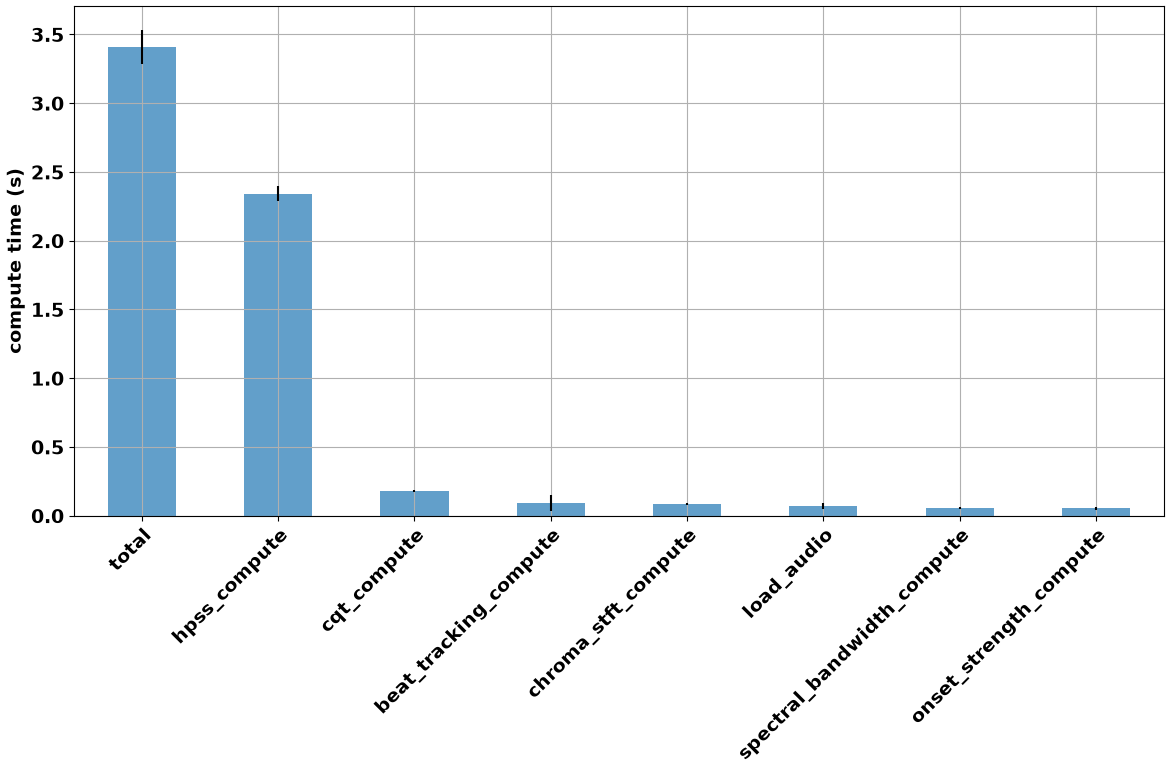
\includegraphics[width=0.88\textwidth]{../../plotting/images/compute_time1.png}
    \caption{The computational time (in seconds) averaged on 200 audio tracks for the 7 most time consuming features. The \texttt{total} bar gives the average total computational time for one track.}
    \label{fig:figure1}
\end{figure}

\begin{figure}
    \centering
    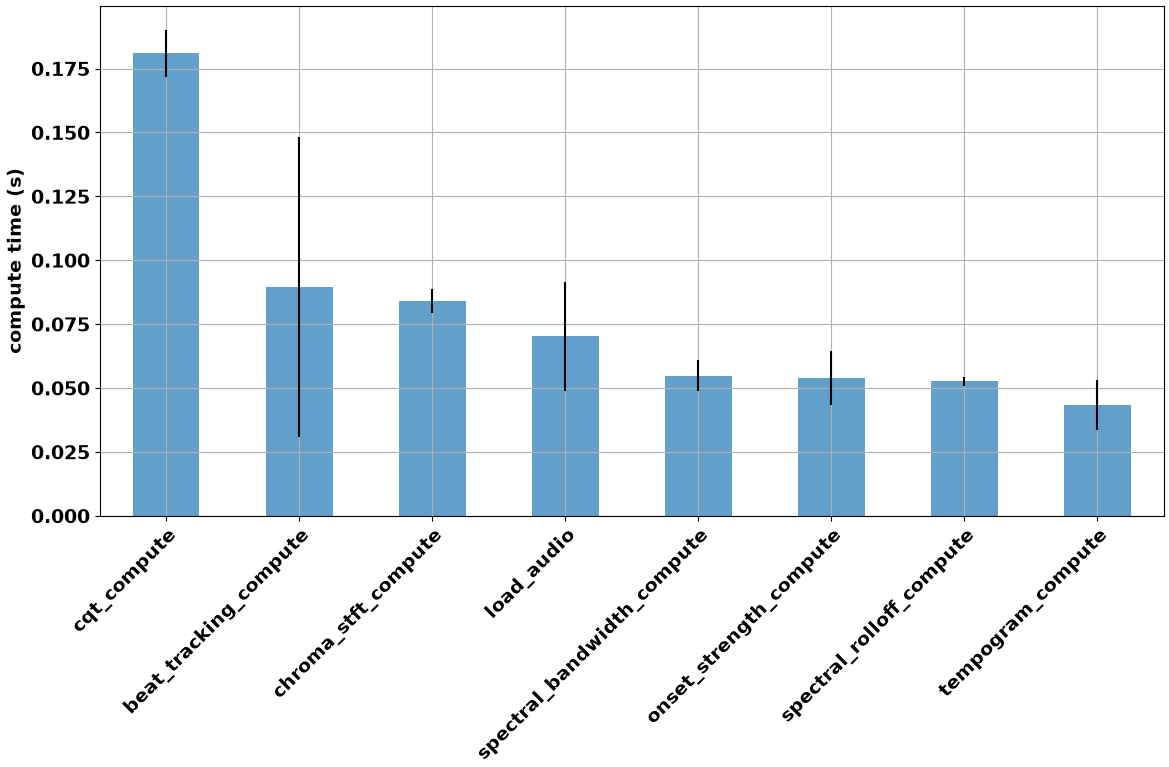
\includegraphics[width=0.88\textwidth]{../../plotting/images/compute_time2.png}
    \caption{The computational time (in seconds) averaged on 200 audio tracks for the most time consuming features. The bars for \texttt{total} and \texttt{hpss\_compute} have been removed to better see the variations on the next columns.}
    \label{fig:figure2}
\end{figure}


\end{document}

%%% Local Variables:
%%% mode: LaTeX
%%% TeX-master: t
%%% End:
